\colorformatcornflowerblue
\setbeamercovered{transparent}

\begin{document}

% -------------------------------------------------------------------------------
% -------------------------------------------------------------------------------

\begin{frame}[plain]
  
\titlepage

\begin{center}

\includegraphics[scale=0.45]{unine}
\end{center}

\end{frame}

% -------------------------------------------------------------------------------
% -------------------------------------------------------------------------------

\subtitle[Introduction]{Introduction}

\begin{frame}{Motivation}
    More and more data needs to be stored reliably on online servers.
    Reliability can be provided through:
    \begin{itemize}
        \item<1> Replication
        \item<1-2> Erasure coding
    \end{itemize}
\end{frame}

\begin{frame}{Motivation}
  \begin{itemize}
  \item  The characteristics of erasure coding algorithms are difficult to evaluate (encoding, decoding, complexity, latency, ...)
  \item  Evaluation is often done theoretically or by simulation
  \end{itemize}

\end{frame}

\begin{frame}{Erasure coding}
    \begin{snugshade}
        Goal: add redundancy to cope with data loss/corruption
    \end{snugshade}

    Example using a $\left(5,2\right)$ Reed-Solomon code:
    \begin{figure}
    \begin{tikzpicture}[transform shape,scale=0.75]
    \draw (1.5,0.5) node[above right] {File contents};
\only<-4,7>{
    \node (d1) at (2,0) [draw,minimum width=1cm,minimum height=1cm] {data};
    \node (d2) at (3,0) [draw,minimum width=1cm,minimum height=1cm] {data};
}
    \node (d3) at (4,0) [draw,minimum width=1cm,minimum height=1cm] {data};
    \node (d4) at (5,0) [draw,minimum width=1cm,minimum height=1cm] {data};
    \node (d5) at (6,0) [draw,minimum width=1cm,minimum height=1cm] {data};
    
\only<3->{
    \node (p1) at (7,0) [blue,draw,minimum width=1cm,minimum height=1cm] {\footnotesize parity};
    \node (p2) at (8,0) [blue,draw,minimum width=1cm,minimum height=1cm] {\footnotesize  parity};
}
    
    \node (algo) at (6.5,-3) [above right,minimum width=1cm,minimum height=1cm,draw,fill=black!10,node contents={algorithm}] {};

\only<2-3>{
    \draw[->,>=stealth,out=270,in=180] (d1.south) to (algo.west);
    \draw[->,>=stealth,out=270,in=180] (d2.south) to (algo.west);
    \draw[->,>=stealth,out=270,in=180] (d3.south) to (algo.west);
    \draw[->,>=stealth,out=270,in=180] (d4.south) to (algo.west);
    \draw[->,>=stealth,out=270,in=180] (d5.south) to (algo.west);
}
\only<3>{
    \draw[->,>=stealth,out=90,in=270] (algo.north) to (p1.south);
    \draw[->,>=stealth,out=90,in=270] (algo.north) to (p2.south);
}
    
\only<6-7>{
    \draw[->,>=stealth,out=270,in=90] (d3.south) to (algo.north);
    \draw[->,>=stealth,out=270,in=90] (d4.south) to (algo.north);
    \draw[->,>=stealth,out=270,in=90] (d5.south) to (algo.north);
    \draw[->,>=stealth,out=270,in=90] (p1.south) to (algo.north);
    \draw[->,>=stealth,out=270,in=90] (p2.south) to (algo.north);
}
\only<7>{
    \draw[->,>=stealth,out=180,in=270] (algo.west) to (d1.south);
    \draw[->,>=stealth,out=180,in=270] (algo.west) to (d2.south);
}
\end{tikzpicture}

    \end{figure}
\end{frame}

\subtitle{Description}

\begin{frame}{\sys \enspace key features}
    \begin{itemize}
        \item Compatible with existing benchmark programs
        \item Automated benchmarks execution
        \item Containerized storage nodes ($>1$ per physical node)
        \item Can replay fault traces
    \end{itemize}
\end{frame}

\begin{frame}{Evaluation example}
    How to evaluate a new erasure coding algorithm
    \begin{enumerate}
        \item Program the algorithm as a Java class
        \item Write benchmarks as Python functions
        \begin{itemize}
            \item Debian-compatible programs can be launched as sub-processes
        \end{itemize}
        \item Configure the evaluation
        \begin{itemize}
            \item e.g. algorithm parameters, fault trace, ...
        \end{itemize}
        \item Easily deploy the solution to a Docker cluster
        \item Collect results
    \end{enumerate}
\end{frame}

\subtitle[Architecture]{Architecture}

\begin{frame}{\sys \enspace technical components}
    \centering
    % TikZ figure showing the relations between all components of the erasure codes tester

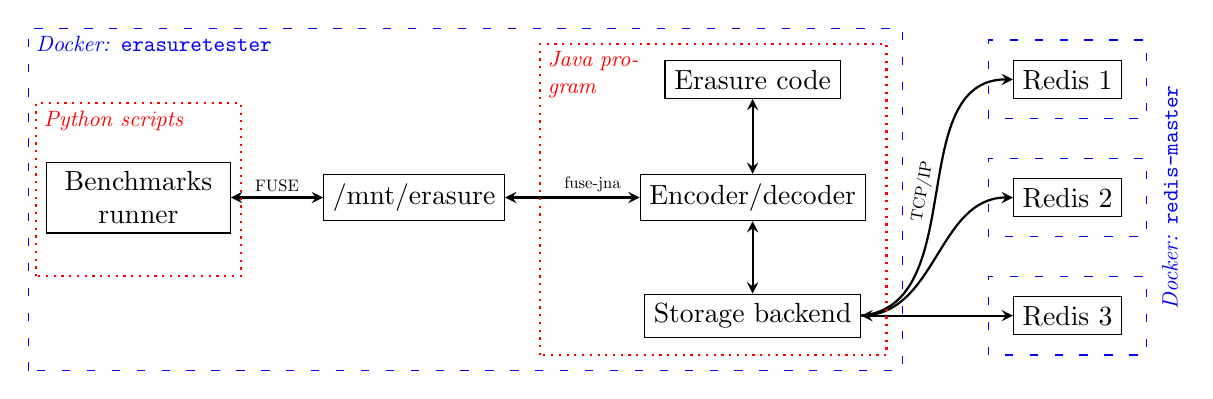
\begin{tikzpicture}
\node[draw, text width=2.1cm, text centered] (bench) at (1.2, 1.5) {Benchmarks runner};
\node[draw] (dir) at (4.7, 1.5) {/mnt/erasure};
\node[draw] (fed) at (9, 1.5) {Encoder/decoder};
\node[draw] (sb) at (9, 0) {Storage backend};
\node[draw] (ec) at (9, 3) {Erasure code};
\node[draw] (r1) at (13, 3) {Redis 1};
\node[draw] (r2) at (13, 1.5) {Redis 2};
\node[draw] (r3) at (13, 0) {Redis 3};

\draw[<->,thick,>=stealth] (bench) -- (dir) node[midway,above,scale=0.6]{FUSE};
\draw[<->,thick,>=stealth] (dir) -- (fed) node[pos=0.65,above,scale=0.6]{fuse-jna};
\draw[<->,thick,>=stealth] (fed) -- (ec);
\draw[<->,thick,>=stealth] (fed) -- (sb);
\draw[->,thick,>=stealth] (sb.east) to[out=5,in=180] node[sloped,midway,scale=0.6,above]{TCP/IP} (r1.west);
\draw[->,thick,>=stealth,out=0,in=180] (sb.east) to[out=0,in=180] (r2.west);
\draw[<->,thick,>=stealth] (sb.east) -- (r3.west);

\draw[loosely dashed,blue] (-0.2,-0.7) rectangle (10.9,3.65);
\draw[loosely dashed,blue] (12,2.5) rectangle (14,3.5);
\draw[loosely dashed,blue] (12,1) rectangle (14,2);
\draw[loosely dashed,blue] (12,-0.5) rectangle (14,0.5);
\draw[dotted,red,thick] (6.3,-0.5) rectangle (10.7,3.45);
\draw[dotted,red,thick] (-0.1,0.5) rectangle (2.5,2.7);

\draw (6.3,3.45) node[below right,red,scale=0.8, text width=1.5cm] {\textit{Java program}};
\draw (-0.1,2.7) node[below right,red,scale=0.8] {\textit{Python scripts}};
\draw (-0.2,3.65) node[below right,blue,scale=0.8] {\textit{Docker:} \texttt{erasuretester}};
\draw (14.3,1.5) node[blue,scale=0.8,rotate=90] {\textit{Docker:} \texttt{redis-master}};
\end{tikzpicture}

\end{frame}

\begin{frame}{Blocks distribution}
    \centering
    % TikZ figure showing how blocks are splitted and encoded

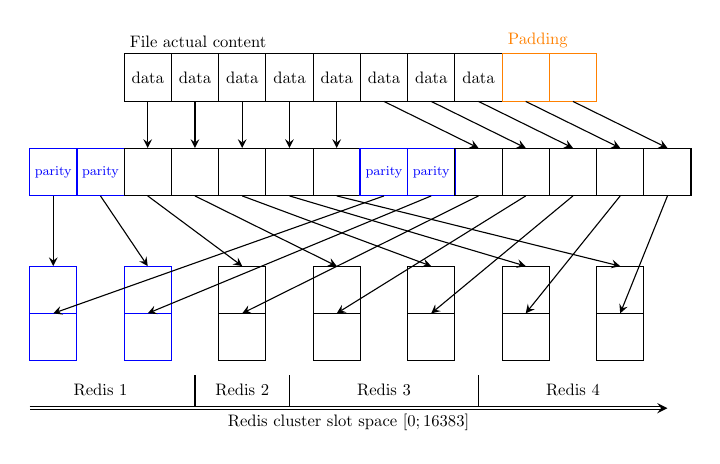
\begin{tikzpicture}[transform shape,scale=0.6]
\draw (1.5,0.5) node[above right] {File actual content};
\node (d1) at (2,0) [draw,minimum width=1cm,minimum height=1cm] {data};
\node (d2) at (3,0) [draw,minimum width=1cm,minimum height=1cm] {data};
\node (d3) at (4,0) [draw,minimum width=1cm,minimum height=1cm] {data};
\node (d4) at (5,0) [draw,minimum width=1cm,minimum height=1cm] {data};
\node (d5) at (6,0) [draw,minimum width=1cm,minimum height=1cm] {data};
\node (d6) at (7,0) [draw,minimum width=1cm,minimum height=1cm] {data};
\node (d7) at (8,0) [draw,minimum width=1cm,minimum height=1cm] {data};
\node (d8) at (9,0) [draw,minimum width=1cm,minimum height=1cm] {data};
\draw (9.5,0.5) node[above right,orange] {Padding};
\node (d9) at (10,0) [orange,draw,minimum width=1cm,minimum height=1cm] {};
\node (d10) at (11,0) [orange,draw,minimum width=1cm,minimum height=1cm] {};

\node (p1) at (0,-2) [draw,minimum width=1cm,minimum height=1cm,blue] {\footnotesize parity};
\node (p2) at (1,-2) [draw,minimum width=1cm,minimum height=1cm,blue] {\footnotesize parity};
\node (p3) at (2,-2) [draw,minimum width=1cm,minimum height=1cm] {};
\node (p4) at (3,-2) [draw,minimum width=1cm,minimum height=1cm] {};
\node (p5) at (4,-2) [draw,minimum width=1cm,minimum height=1cm] {};
\node (p6) at (5,-2) [draw,minimum width=1cm,minimum height=1cm] {};
\node (p7) at (6,-2) [draw,minimum width=1cm,minimum height=1cm] {};
\node (p8) at (7,-2) [draw,minimum width=1cm,minimum height=1cm,blue] {\footnotesize parity};
\node (p9) at (8,-2) [draw,minimum width=1cm,minimum height=1cm,blue] {\footnotesize parity};
\node (p10) at (9,-2) [draw,minimum width=1cm,minimum height=1cm] {};
\node (p11) at (10,-2) [draw,minimum width=1cm,minimum height=1cm] {};
\node (p12) at (11,-2) [draw,minimum width=1cm,minimum height=1cm] {};
\node (p13) at (12,-2) [draw,minimum width=1cm,minimum height=1cm] {};
\node (p14) at (13,-2) [draw,minimum width=1cm,minimum height=1cm] {};

\draw[->,>=stealth] (d1.south) to (p3.north);
\draw[->,>=stealth] (d2.south) to (p4.north);
\draw[->,>=stealth] (d3.south) to (p5.north);
\draw[->,>=stealth] (d4.south) to (p6.north);
\draw[->,>=stealth] (d5.south) to (p7.north);
\draw[->,>=stealth] (d6.south) to (p10.north);
\draw[->,>=stealth] (d7.south) to (p11.north);
\draw[->,>=stealth] (d8.south) to (p12.north);
\draw[->,>=stealth] (d9.south) to (p13.north);
\draw[->,>=stealth] (d10.south) to (p14.north);

\node (r1) at (0,-4.5) [blue,draw,minimum width=1cm,minimum height=1cm] {};
\node (r2) at (2,-4.5) [blue,draw,minimum width=1cm,minimum height=1cm] {};
\node (r3) at (4,-4.5) [draw,minimum width=1cm,minimum height=1cm] {};
\node (r4) at (6,-4.5) [draw,minimum width=1cm,minimum height=1cm] {};
\node (r5) at (8,-4.5) [draw,minimum width=1cm,minimum height=1cm] {};
\node (r6) at (10,-4.5) [draw,minimum width=1cm,minimum height=1cm] {};
\node (r7) at (12,-4.5) [draw,minimum width=1cm,minimum height=1cm] {};

\node (r8) at (0,-5.5) [blue,draw,minimum width=1cm,minimum height=1cm] {};
\node (r9) at (2,-5.5) [blue,draw,minimum width=1cm,minimum height=1cm] {};
\node (r10) at (4,-5.5) [draw,minimum width=1cm,minimum height=1cm] {};
\node (r11) at (6,-5.5) [draw,minimum width=1cm,minimum height=1cm] {};
\node (r12) at (8,-5.5) [draw,minimum width=1cm,minimum height=1cm] {};
\node (r13) at (10,-5.5) [draw,minimum width=1cm,minimum height=1cm] {};
\node (r14) at (12,-5.5) [draw,minimum width=1cm,minimum height=1cm] {};


\draw[->,>=stealth] (p1.south) to (r1.north);
\draw[->,>=stealth] (p2.south) to (r2.north);
\draw[->,>=stealth] (p3.south) to (r3.north);
\draw[->,>=stealth] (p4.south) to (r4.north);
\draw[->,>=stealth] (p5.south) to (r5.north);
\draw[->,>=stealth] (p6.south) to (r6.north);
\draw[->,>=stealth] (p7.south) to (r7.north);
\draw[->,>=stealth] (p8.south) to (r8.north);
\draw[->,>=stealth] (p9.south) to (r9.north);
\draw[->,>=stealth] (p10.south) to (r10.north);
\draw[->,>=stealth] (p11.south) to (r11.north);
\draw[->,>=stealth] (p12.south) to (r12.north);
\draw[->,>=stealth] (p13.south) to (r13.north);
\draw[->,>=stealth] (p14.south) to (r14.north);

\node (redis1) at (1,-6.6) {Redis 1};
\draw (3,-6.3) to (3,-6.95);
\node (redis1) at (4,-6.6) {Redis 2};
\draw (5,-6.3) to (5,-6.95);
\node (redis1) at (7,-6.6) {Redis 3};
\draw (9,-6.3) to (9,-6.95);
\node (redis1) at (11,-6.6) {Redis 4};
\draw[->,>=stealth,double] (-0.5,-7) to node[midway,below]{Redis cluster slot space $\left[0;16383\right]$} (13,-7);

\end{tikzpicture}

\end{frame}

\begin{frame}{\sys\enspace metadata management}
  \begin{itemize}
  \item Each block is identified by a 32-bit key. Using it, we derive:
    \begin{enumerate}
        \item Key of the blocks aggregation stored in Redis
        \item Offset within that aggregation
    \end{enumerate}
    
    \item The list of all block keys is kept in memory

  \end{itemize}
\end{frame}

\begin{frame}{\sys\enspace automated deployment and scaling}
  \begin{snugshade}
    As part of \sys, we provide scripts that automate the deployment of the solution to a Docker Swarm cluster, up to the collection of results
  \end{snugshade}
\end{frame}

\subtitle[Evaluation]{Evaluation}

\begin{frame}{Evaluation}
    We evaluated algorithms from the following paper:

    \begin{snugshade}
        \footnotesize
        M.~Sathiamoorthy, M.~Asteris, D.~Papailiopoulos, A.~G.~Dimakis, R.~Vadali, S.~Chen, and D.~Borthakur, “XORing elephants: Novel erasure codes for big data,” in Proceedings of the VLDB Endowment, vol. 6, 2013, pp. 325–336.
    \end{snugshade}
    
    \begin{description}
        \item[NC] No erasure coding
        \item[RS] $(10,4)$ Reed-Solomon code
        \item[LRC] $(10,6,5)$ Locally Repairable Code
    \end{description}
\end{frame}

\begin{frame}{Throughput}
    \begin{figure}
        \begin{tikzpicture}
\usetikzlibrary{plotmarks}
\pgfplotsset{width=\linewidth, height=7cm}
\begin{groupplot}[
    group style={
        group size=2 by 2,
        vertical sep=0pt,
        horizontal sep=0pt,
        xlabels at=edge bottom,
        ylabels at=edge left,
        xticklabels at=edge bottom,
        yticklabels at=edge left
    },
    ymin=0,
    width=\linewidth / 1.9,
    enlarge x limits=0.3,
    ybar=3.5mm,
    nodes near coords,
    every node near coord/.append style={
        rotate=90,
        anchor=north,
        font=\footnotesize,
        xshift=4.5mm
    },
    xtick=data,
    xlabel=File size,
    ylabel={Throughput $\left[\text{kB/s}\right]$},
    symbolic x coords={4 MB, 16 MB, 64 MB}
]
\nextgroupplot[ymax=4700]
% Write with FUSE
\addplot+[error bars/.cd,y dir=both, y explicit] coordinates {
    % Write Null
    (4 MB, 1590) +- (0, 31.62)
    (16 MB, 1160) +- (0, 51.64)
    (64 MB, 579) +- (0, 7.38)
};
\addplot+[error bars/.cd,y dir=both, y explicit] coordinates {
    % Write RS
    (4 MB, 1090) +- (0, 32.91)
    (16 MB, 770) +- (0, 17.21)
    (64 MB, 392) +- (0, 2.90)
};
\addplot+[error bars/.cd,y dir=both, y explicit] coordinates {
    % Write LRC
    (4 MB, 998) +- (0, 4.37)
    (16 MB, 670) +- (0, 10.28)
    (64 MB, 340) +- (0, 1.41)
};

\legend{Null, \acs{rs}, \acs{lrc}}

% Write direct
\nextgroupplot[ymax=4700]
\addplot+[error bars/.cd,y dir=both, y explicit] coordinates {
    % Write Null
    (4 MB, 2999) +- (0, 824.6)
    (16 MB, 3536) +- (0, 289.1)
    (64 MB, 3838) +- (0, 81.1)
};
\addplot+[error bars/.cd,y dir=both, y explicit] coordinates {
    % Write RS
    (4 MB, 1743) +- (0, 235.5)
    (16 MB, 1874) +- (0, 481.6)
    (64 MB, 2084) +- (0, 264.5)
};
\addplot+[error bars/.cd,y dir=both, y explicit] coordinates {
    % Write LRC
    (4 MB, 1502) +- (0, 287.6)
    (16 MB, 1632) +- (0, 301.6)
    (64 MB, 1817) +- (0, 197.3)
};

\nextgroupplot[ymax=2450]
% Read with FUSE
\addplot+[error bars/.cd,y dir=both, y explicit] coordinates {
    % Read Null
    (4 MB, 930) +- (0, 29.22)
    (16 MB, 1120) +- (0, 43.87)
    (64 MB, 1530) +- (0, 50.26)
};
\addplot+[error bars/.cd,y dir=both, y explicit] coordinates {
    % Read RS
    (4 MB, 711) +- (0, 13.06)
    (16 MB, 891) +- (0, 40.30)
    (64 MB, 1100) +- (0, 0)
};
\addplot+[error bars/.cd,y dir=both, y explicit] coordinates {
    % Read LRC
    (4 MB, 791) +- (0, 17.56)
    (16 MB, 1011) +- (0, 50.67)
    (64 MB, 1130) +- (0, 50.26)
};

% Read direct
\nextgroupplot[ymax=2450]
\addplot+[error bars/.cd,y dir=both, y explicit] coordinates {
    % Read Null
    (4 MB, 1497) +- (0, 543.6)
    (16 MB, 1899) +- (0, 71.2)
    (64 MB, 1907) +- (0, 34.1)
};
\addplot+[error bars/.cd,y dir=both, y explicit] coordinates {
    % Read RS
    (4 MB, 1116) +- (0, 411.9)
    (16 MB, 1442) +- (0, 44.8)
    (64 MB, 1419) +- (0, 58.7)
};
\addplot+[error bars/.cd,y dir=both, y explicit] coordinates {
    % Read LRC
    (4 MB, 1296) +- (0, 432.4)
    (16 MB, 1632) +- (0, 24.0)
    (64 MB, 1599) +- (0, 33.1)
};
\end{groupplot}

\node[anchor=north] at (group c1r1.north) {\acs{fuse} write};
\node[anchor=north] at (group c1r2.north) {\acs{fuse} read};
\node[anchor=north] at (group c2r1.north) {Direct write};
\node[anchor=north] at (group c2r2.north) {Direct read};
\end{tikzpicture}

    \end{figure}
\end{frame}

\begin{frame}{Traffic}
    \begin{figure}
        \begin{tikzpicture}
\usetikzlibrary{plotmarks}
\pgfplotsset{every axis plot post/.append style={
        solid,
        mark size=1.7pt
    },
    height=6.5cm,
    width=\linewidth,
}
\begin{axis}[
    xlabel={Elapsed time $\left[\si{\second}\right]$},
    ylabel={Network throughput $\left[\si{\mega\byte\per\second}\right]$},
    ymax=34000000,
    cycle list name=exotic,
    cycle list shift=1,
    legend style={
        anchor=north,
        at={(0.5,0.97)},
    },
    legend cell align=left,
    legend columns=2,
    scaled y ticks=base 10:-6,
    ytick scale label code/.code={},
]
\addplot table[x=x, y=write-100nodes-ReedSolomon] {plots/throughput.dat};
\addplot table[x=x, y=write-100nodes-SimpleRegenerating] {plots/throughput.dat};
\addplot table[x=x, y=read-normal-100nodes-ReedSolomon] {plots/throughput.dat};
\addplot table[x=x, y=read-normal-100nodes-SimpleRegenerating] {plots/throughput.dat};
\addplot table[x=x, y=read-degraded-100nodes-ReedSolomon] {plots/throughput.dat};
\addplot table[x=x, y=read-degraded-100nodes-SimpleRegenerating] {plots/throughput.dat};

\legend{RS write, LRC write, RS read, LRC read, RS deg. read, LRC deg. read}
\end{axis}
\end{tikzpicture}

    \end{figure}
\end{frame}

\begin{frame}{Trace}
    \begin{figure}
        %\pgfplotstabletypeset[string type]{plots/websites-size.dat}

\begin{tikzpicture}
\usetikzlibrary{plotmarks}
\pgfplotsset{width=\linewidth, height=7cm,
    every axis plot post/.append style={
        solid,
        thin,
        mark=none
    }
}
\begin{axis}[
    date coordinates in=x,
    xlabel=Date,
    ylabel=Available nodes,
    table/col sep=comma,
    x tick label style={rotate=20}
]
\addplot+ table[x=date, y=size] {plots/websites-size.dat};
\end{axis}
\end{tikzpicture}

    \end{figure}
\end{frame}

\subtitle[Conclusion]{Conclusion}

\begin{frame}{Conclusion}

  \begin{snugshade}
    Using \sys, evaluating an erasure coding algorithm under real conditions is easier and cheaper
  \end{snugshade}
  
  \begin{snugshade}
    Available open-source at \url{https://github.com/safecloud-project/erasurebench}    
  \end{snugshade}

\end{frame}

% -------------------------------------------------------------------------------
% -------------------------------------------------------------------------------

\end{document}

% -------------------------------------------------------------------------------
